\chapter{Analysis of differences} \label{Chp:Verschil}

Here we compare the results of \dfastmi using the new \emph{stepped-hydrograph} approach with the results of the classic 3-discharge approach of \dfmi 2 / WAQMORF.
The purpose of this comparison is to verify that the results are similar when both methods are used as intended.
For this purpose the following cases are currently used:

\begin{itemize}
\item \nameref{Sec:GendtseWaard}
%\item Rijntakken II
%\item Rijntakken III (optioneel)
\item \nameref{Sec:DeLymen}
\end{itemize}

The additional simulations required for the new \emph{stepped-hydrograph} method have been carried out using the same schematisation and software versions as used in the original analysis.

%	Evt. kunnen we alles met de nieuwste versies schematiseren en doorrekenen; in dat geval kan er mogelijk ook een verschilanalyse gedaan worden met een voorgaande software-versie.


\section{Gendtse Waard}\label{Sec:GendtseWaard}

\emph{The input files of this case are included in the distribution under \file{examples/03 - Gendtse Waard}.}

This concerns a secondary channel located at the "Gendtse Waard" along the Bovenwaal, a stretch of the river Waal.
This case is also used for the backward compatibility tests, see \autoref{Sec:GendtseWaard_backward}.
In the backward compatibility mode \dfmi uses the flow fields at 3000, 4000, and \SI{6000}{\metre\cubed\per\second} at Lobith.
For the new analysis, this list is extended with 1300, 2000, and \SI{8000}{\metre\cubed\per\second}.
Furthermore, the bed celerity has changed.
In the backward compatibility mode the algorithms use for the Boven-Waal \SI{0.81}{\kilo\metre\per\year} at a discharge of \SI{3000}{\metre\cubed\per\second}, and \SI{3.65}{\kilo\metre\per\year} at 4000 and \SI{6000}{\metre\cubed\per\second}.
The celerity at the Boven-Waal equals 0.63, 0.97, 1.51, 2.06, 3.16 and \SI{5.35}{\kilo\metre\per\year} at a discharge of 1300, 2000, 3000, 4000, 6000, and \SI{8000}{\metre\cubed\per\second}, respectively, for the new analysis.
The discharge statistics (exceedance curve) has not changed.

\begin{figure}[h]
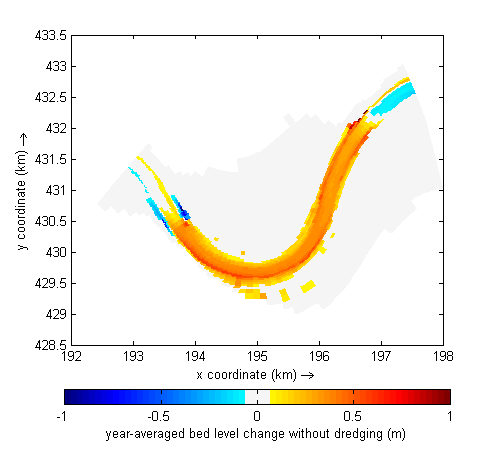
\includegraphics[width=\columnwidth/2]{figures/report_Figure1_QP.png}
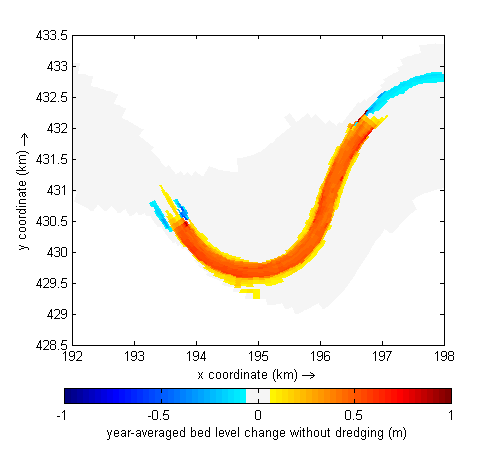
\includegraphics[width=\columnwidth/2]{figures/report_Figure1_v3_QP.png}
\caption{Morphological impact as computed by \dfmi version 3 in backward compatibility mode (left; same as WAQMORF) and in the new default mode (right).
Visualized using QUICKPLOT.}
\label{GendtseWaard_diff}
\end{figure}

The results of the WAQMORF-compatible analysis and the new analysis method are presented side-by-side in \autoref{GendtseWaard_diff}.
The indicated year-averaged equilibrium sedimentation is on average slightly higher than before.
This will have only a minor effect on the estimated sedimentation volume after one year since it is offset by a slightly reduced impacted length.
The impacted length is \SI{1043}{\metre} for the new analysis method, compared to \SI{1319}{\metre} using the old analysis method.
Overall, the new method gives a result that closely resembles the results previously obtained using WAQMORF (or the backward compatibility mode of \dfmi).

\section{De Lymen}\label{Sec:DeLymen}
This concerns a section of the "Bedijkte Maas" between Batenburg and Appeltern, along the river Meuse.
This case is also used for the backward compatibility tests, see \autoref{Sec:DeLymen_backward}.

The new simulations for this case have not yet been completed as this requires a decision regarding the use of regular steady-state simulations (so-called S-runs) or steady-state simulations corrected for dynamic ("topvervlakking") effects (so-called SD-runs) and derivation of the associated boundary conditions and laterals.

%\todo{Run WAQUA for 1300, 1700, 2100, 2500, and 3200 \SI{}{\metre\cubed\per\second} at Borgharen}

%The results of the WAQMORF-compatible analysis and the new analysis method are presented side-by-side in \autoref{Lymen_diff}.
%Both methods give similar results.

%\begin{figure}
%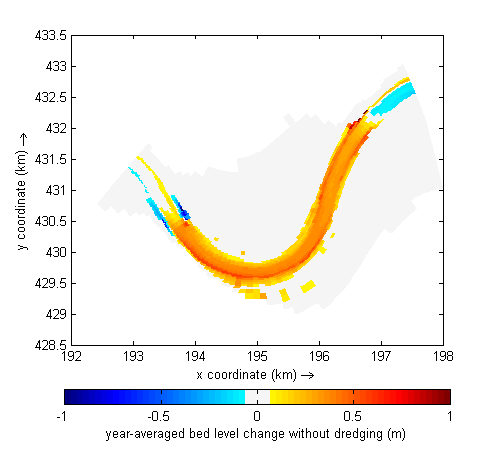
\includegraphics[width=\columnwidth/2]{figures/report_Figure1_QP.png}
%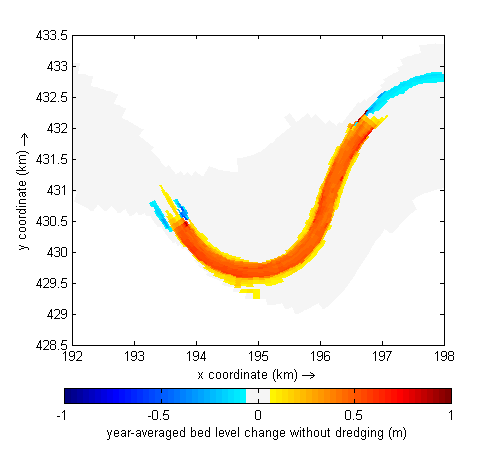
\includegraphics[width=\columnwidth/2]{figures/report_Figure1_v3_QP.png}
%\caption{Morphological impact as computed by \dfmi version 3 in backward compatibility mode (left; same as WAQMORF) and in the new default mode (right).
%Visualized using QUICKPLOT.}
%\label{Lymen_diff}
%\end{figure}